\documentclass[%
		%draft,
    %submission,
    %compressed,
    final,
    %
    %technote,
    %internal,
    %submitted,
    %inpress,
    reprint,
    %
    %titlepage,
    notitlepage,
    %anonymous,
    narroweqnarray,
    inline,
    twoside,
    invited
    ]{ieee}

\usepackage[utf8]{inputenc}
\usepackage[spanish]{babel}
\usepackage{graphicx}
\usepackage{verbatim}
\usepackage{moreverb}
\usepackage{amsmath}
\usepackage{amsfonts}
\usepackage{amssymb}
\usepackage{fancybox}
\usepackage{float}
\usepackage{fancyvrb}
\usepackage{subfigure}

\newcommand{\latexiie}{\LaTeX2{\Large$_\varepsilon$}}

%\usepackage{ieeetsp}    % if you want the "trans. sig. pro." style
%\usepackage{ieeetc}    % if you want the "trans. comp." style
%\usepackage{ieeeimtc}    % if you want the IMTC conference style

% Use the `endfloat' package to move figures and tables to the end
% of the paper. Useful for `submission' mode.
%\usepackage {endfloat}

% Use the `times' package to use Helvetica and Times-Roman fonts
% instead of the standard Computer Modern fonts. Useful for the 
% IEEE Computer Society transactions.
%\usepackage{times}
% (Note: If you have the commercial package `mathtime,' (from 
% y&y (http://www.yandy.com), it is much better, but the `times' 
% package works too). So, if you have it...
%\usepackage {mathtime}

% for any plug-in code... insert it here. For example, the CDC style...
%\usepackage{ieeecdc}

\begin{document}

%----------------------------------------------------------------------
% Title Information, Abstract and Keywords
%----------------------------------------------------------------------
\title[Algoritmos Genéticos]{%
       Algoritmos Genéticos}

% format author this way for journal articles.
% MAKE SURE THERE ARE NO SPACES BEFORE A \member OR \authorinfo
% COMMAND (this also means `don't break the line before these
% commands).
\author[Castiglione, Karpovsky, Sturla]{Gonzalo V. Castiglione, Alan E. Karpovsky, Martín Sturla\\\textit{Estudiantes 
       Instituto Tecnológico de Buenos Aires (ITBA)}\\
\textbf{12 de Junio de 2012}
}


\journal{Cátedra\ \ Sist.\ de\ Inteligencia\ Artificial,\ ITBA\ }
\titletext{-\ 12, JUNIO\ 2012}
\ieeecopyright{\copyright\ 2012 ITBA}
\lognumber{}
\pubitemident{}
\loginfo{12 de Junio, 2012.}
\firstpage{1}

\confplacedate{Buenos Aires, Argentina, 12 de Junio, 2012}

\maketitle               

\begin{abstract} 
El presente informe busca analizar la utilización de algoritmos genéticos para la obtención de pesos de redes neuronales multicapa. Se estudiarán distintas técnicas de selección, cruza, mutación y reemplazo de los individuos y se detallarán los resultados obtenidos.
\end{abstract}

\begin{keywords}
algotitmos genéticos, métodos de selección, métodos de cruza, redes neuronales, evolución, población, mutación, reemplazo, individuo, gen
\end{keywords}

%----------------------------------------------------------------------
% SECTION I: Introduccion%----------------------------------------------------------------------
\section{Introducción}

\par Se analizó el comportamiento de los algoritmos genéticos en el problema de la obtención de pesos para redes neuronales multicapa.\\
Con este fin se implementó un algoritmo que permite definir de manera sencilla todos los parámetros más importantes del motor de algoritmos genéticos con el fin de hacer más simple y práctico su estudio. Los parámetros que el usuario puede modificar son los siguientes:\\

\begin{itemize} 
\item Tamaño de la población $(N)$
\item Brecha generacional $(G)$
\item Número máximo de generaciones
\item Probabilidad de mutación $(p_m)$
\item Probabilidad de cruce $(p_c)$
\item Método de selección
\item Método de reemplazo
\end{itemize} 


%----------------------------------------------------------------------
% SECTION II: Marco Teórico
%----------------------------------------------------------------------

\section{Desarrollo}

\subsection{Modelado del problema}

\subsubsection{Representación de los individuos}

\par Se decidio representar a cada individuo de la población (red neuronal multicapa en este caso) de la siguiente forma: Cada capa de la red neuronal está represnetada por un arreglo de pesos; por consiguiente una red neuronal es la concatenación de los arreglos de cada una de sus capas. Un cromosoma será entonces un arreglo en el que cada locus representará un peso puntual de la red.

\subsubsection{Diagramación del algoritmo}

\par En lo que a algoritmos genéticos respecta, existen numerosas formas de pensar la diagramación del mismo. Si bien la base teórica de fondo siempre es la misma, la forma en la que se eligen los individuos para ser cruzados, la forma en la que los individuos cruzados pasan o no pasan a la siguiente generación y demás aspectos pueden quedar a elección de quien sea que implemente el motor de algoritmos genéticos.\\
\par En la \textbf{Figura 1} del \textbf {Anexo A} se observa el modelado elegido para la implementación del algoritmo: \\\\
Suponiendo poblaciones de 10 individuos y un gap generacional $G = 0.6$ se seleccionan, mediante alguno de los métodos de selección que desarrollaremos a continuación, un $(G*100)\%$ de la cantidad de individuos $(N)$ de la \textit{generación i}. Es decir que para el ejemplo de poblaciones de 10 individuso y $G = 0.6$, se tomarán $6$ individuos (un $60\%$ del tamaño de la población). Estos $6$ individuos seleccionados son cruzados mediante alguno de los métodos de \textit{crossover} y luego son pasados directamente a la \textit{generación i+1} con cierta probabilidad de mutación y/o de \textit{backpropagation}. Esto quiere decir que con cierta probabilidad baja, los hijos de los individuos seleccionados pueden ser mutados y/o entregandos mediante \textit{backpropagation} antes de ser pasados a la próxima generación.\\\\
De esta forma, la \textit{generación i+1} ya tiene $6$ de los $10$ individuos necesarios. Los $4$ individuos restantes son seleccionados de entre los $10$ individuos de la \textit{generación i}; en otras palabras son seleccionados entre los padres de los hijos obtenidos por la cruza y los que nunca fueron elegidos en un principio por el método de selección. Nótese que los $4$ individuos en cuestión del ejemplo son seleccionados mediante los métodos de reemplazo.\\

\par El motor de algoritmos genéticos implementado tiene la particularidad de permitir el uso de métodos mixtos para la selección y el reemplazo de los individuos. El usuario puede optar por elegir los individuos a cruzar bajo el método de selección \textit{Elite} y luego elegir los individuos a reemplazar utilizando \textit{Ruleta}.

\subsection{Función de fitness}

\par La función de \textit{fitness} mide el grado de adaptación de un determinado individuo al entorno actual. Para este problema en particular se optó por tomar como función de \textit{fitness} $f(i) = \frac{1}{ECM}$ siendo $i$ una red neuronal (individuo) y $ECM$ el error cuadrático medio obtenido al evaluar la misma.

\section{Métodos de selección y reemplazo}

\par Los métodos de selección y reemplazo son utilizados, valga la redundancia, para seleccionar los individuos de una determinada población. El \textit{input} de este tipo de métodos es básicamente una población y algún parámetro de configuración (como ser la brecha generacional) y el \textit{output} de éstos es un conjunto determinado de individuos.

\subsection{Elite}

\par El método de selección/reemplazo \textit{Elite} consiste en elegir a los $k$ ``mejores'' individuos de la población, considerando mejores a los individuos con mejor \textit{fitness}.

\subsection{Ruleta}

\par La selección/reemplazo por ruleta se realiza de la siguiente manera:\\

\begin{enumerate}

\item Se evalúa el fitness, $fi$, de cada individuo de la población.
\item Se computa la probabilidad \textit{(slot size)}, $p_i$, de seleccionar al miembio $i$ de la población:	$p_i=\frac{f_i}{\sum_{j=1}^{N}{f_j}}$, donde $N$ es el tamaño de la población.
\item Calcular la probabilidad acumulada, $q_i$, para cada individuo: $q_i=\sum_{j=1}^{i}{p_j}$.
\item Generar un número \textit{random}, $r \in (0, 1]$.
\item Si $r < q_1$ entonces seleccionar al primer cromosoma, $x_1$. Sino seleccionar al individuo $x_i$ tal que $q_{i-1} < r \leq q_i$. 
\item Repetir los pasos 4 y 5 $k$ veces para crear $k$ candidatos seleccionados.
\end{enumerate}

\subsection{Boltzman}

\par La selección/reemplazo por Boltzman estipula que la probabilidad de ser elegido es proporcional a una funcioón no lineal del \textit{fitness} y de la ``temperatura''. En este sentido guarda ciertas similitudes a \textit{simmulated annealed}: al principio busca diversidad y luego baja la temperatura haciedno que cada vez haya menos diveridad de acuerdo a cierto decrease rate.

\subsection{Torneo}

En la selección/reemplazo por torneo se procede de la siguiente forma:

\begin{enumerate}
\item Se eligen 2 individuos al azar. 
\item Se toma un número \textit{random} $r \in [0, 1]$.
\item Si $r < 0.75$ se seleciona al más apto (de mayor \textit{fitness}), sino se selecciona al menos apto.
\item Ambos individuos se devuelven a la población original y podrían ser seleccionados nuevamente.
\end{enumerate}

\subsection{Universal}

\par La selección universal estocástica se asimila mucho a ruleta pero a diferencia de ésta se genera un solo $r \in [0, \frac{F}{k}]$ para elegir $k$ individuos.  Se tiene a su vez que $r_j = \frac{r + j-1}{k}$ con $j \in [1,k]$.

\subsection{Mixto}

La selección/reemplazo mixto consiste en elegir $k_e$ individuos utilizando \textit{Elite} (ke es ingresado como parámetro) y el resto de los individuos por \textit{Ruleta / Boltzman}.

\section{Criterios de corte}

\par Los criterios de corte implementados son los siguientes:\\

\begin{itemize}
\item \textbf{Máxima cantidad de generaciones:} Dado un número $p$, el algoritmo termina al alcanzarse $p$ generaciones.
\item \textbf{Entorno al óptimo:} Se llega a la solución óptima o se alcanza un fitness superior a una determinada cota.
\item \textbf{Contenido:} Se corta al detectar que el mejor fitness de la población no progresa con las generaciones.
\item \textbf{Estructura:} Se finaliza al detectar que una parte relevante de la poblacioón no cambia de generacioón en generación. Es decir, dado un porcentaje $p$, el algoritmo termina cuando la cantidad de individuos iguales de la generación es mayor a dicho $p$.
\end{itemize}

\section{Mutación y backpropagation}

\par Una vez cruzados, los individuos pasan a la siguiente generación con una probabilidad baja de ser mutados y/o entrenados mediante \textit{backpropagation}.\\
\par La mutación se realiza de la siguiente manera: Se toma un peso al azar del individuo y se le suma un número random proporcional al valor del mismo. Es decir, se le agrega cierto ruido a uno de los pesos de la red neuronal en cuestión.

\section{Resultados}

\section{Conclusión}


%----------------------------------------------------------------------


\clearpage
\onecolumn

\section*{Anexo A: Gráficos}

\begin{figure}[H]
\begin{center}
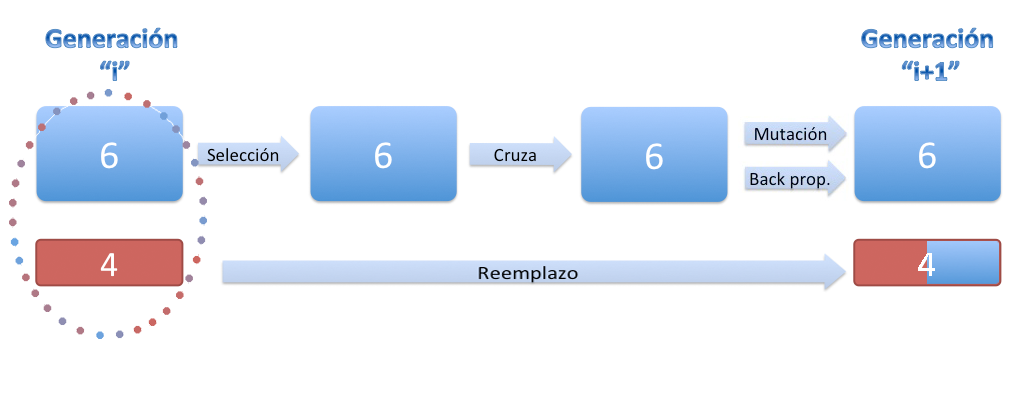
\includegraphics[scale=1.90]{./images/AlgGenModelado.png}
\label{modelado}
\end{center}
\end{figure}

\begin{center}
\par Figura 1: Modelado esquemático del funcionamiento del algoritmo genético para poblaciones de 10 individuos y un gap generacional G = 0.6.
\end{center}


%\VerbatimInput{./code/calculoAb.m}




\end{document}